\begin{center}
    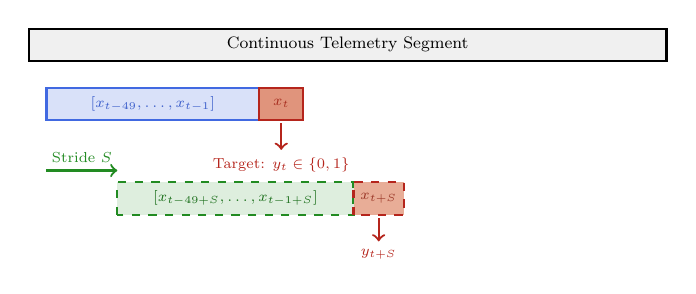
\begin{tikzpicture}[scale=0.75, every node/.style={transform shape}]
        \draw[thick, fill=gray!12] (0, 0) rectangle (10.8, 0.55);
        \node at (5.4, 0.28) {\footnotesize Continuous Telemetry Segment};

        \draw[thick, RoyalBlue, fill=RoyalBlue!20] (0.3, -1.0) rectangle (3.9, -0.45);
        \draw[thick, BrickRed, fill=BrickRed!40] (3.9, -1.0) rectangle (4.65, -0.45);
        \node[RoyalBlue!90!black] at (2.1, -0.72) {\scriptsize $[x_{t-49}, \dots, x_{t-1}]$};
        \node[BrickRed!90!black] at (4.275, -0.72) {\scriptsize $x_t$};
        
        \draw[->, thick, BrickRed] (4.275, -1.05) -- (4.275, -1.5) node[below] {\scriptsize Target: $y_t \in \{0, 1\}$};

        \draw[->, thick, ForestGreen] (0.3, -1.85) -- (1.5, -1.85) node[midway, above] {\scriptsize Stride $S$};

        \draw[thick, dashed, ForestGreen, fill=ForestGreen!15] (1.5, -2.6) rectangle (5.5, -2.05);
        \draw[thick, dashed, BrickRed, fill=BrickRed!30] (5.5, -2.6) rectangle (6.35, -2.05);
        \node[ForestGreen!80!black] at (3.5, -2.32) {\scriptsize $[x_{t-49+S}, \dots, x_{t-1+S}]$};
        \node[BrickRed!80!black] at (5.925, -2.32) {\scriptsize $x_{t+S}$};
        \draw[->, thick, BrickRed] (5.925, -2.65) -- (5.925, -3.05) node[below] {\scriptsize $y_{t+S}$};
    \end{tikzpicture}
\end{center}